\section{Chương 2: Cơ Sở Lý Thuyết và Ý Nghĩa Các Đặc Trưng}
\subsection{Mô hình ảnh và quy ước tọa độ}
Ảnh xám được mô tả bởi hàm cường độ $I(x,y)$; trên máy tính, ảnh là ma trận $I[j,i]$ với cột $i$ tương ứng trục $x$ và hàng $j$ tương ứng trục $y$. Trong dự án, $x$ tăng sang phải và $y$ tăng xuống dưới. Quy ước này cần được giữ giữa Python và Fiji: đổi hàng với cột sẽ hoán đổi $L_x,L_y$; đổi hướng trục có thể đổi dấu đạo hàm bậc lẻ dù hình dạng đáp ứng vẫn giống nhau.

Với ảnh màu, phép phân tích được thực hiện trên ảnh xám đã chuẩn hóa của bộ dữ liệu. Đặc biệt, ảnh DRIVE dùng trong repo đã được chuẩn bị cho bài toán mạch máu; không áp dụng thêm một phép chuyển đổi màu tùy ý cho riêng một nhánh. Cả hai bộ cài đặt phải đọc cùng dữ liệu đầu vào, cùng kích thước và cùng miền cường độ.

\subsection{Gaussian smoothing: công thức và vai trò}
Hạt nhân Gaussian hai chiều đẳng hướng có dạng
\begin{equation}
G_\sigma(x,y)=\frac{1}{2\pi\sigma^2}
\exp\left(-\frac{x^2+y^2}{2\sigma^2}\right),\qquad \sigma>0.
\label{eq:gaussian2d}
\end{equation}
Ảnh làm mịn được xác định bởi
\begin{equation}
L(x,y;\sigma)=(G_\sigma*I)(x,y).
\label{eq:scalespace}
\end{equation}
Mỗi pixel đầu ra là trung bình có trọng số của vùng lân cận; điểm gần tâm có trọng số lớn hơn điểm xa tâm. Vì $\int G_\sigma\,dx\,dy=1$, lọc Gaussian bảo toàn một ảnh hằng trong mô hình liên tục. Khi rời rạc hóa, tổng các hệ số kernel cần được chuẩn hóa về 1 để giữ tính chất tương ứng.

Tham số $\sigma$ là độ lệch chuẩn, đo bằng pixel nếu ảnh chưa hiệu chuẩn kích thước vật lý. $\sigma$ càng lớn, vùng lấy trung bình càng rộng: nhiễu và các biến thiên nhỏ giảm đi, nhưng ranh giới và chi tiết mảnh cũng có thể mờ hơn. Vì vậy làm mịn là một sự đánh đổi giữa ổn định trước nhiễu và bảo toàn độ phân giải không gian.

\subsubsection{Tính khả tách và chi phí tính toán}
Đặt $g_\sigma(x)=\exp(-x^2/2\sigma^2)/(\sqrt{2\pi}\sigma)$, ta có $G_\sigma(x,y)=g_\sigma(x)g_\sigma(y)$. Từ tính kết hợp của tích chập,
\begin{equation}
I*G_\sigma=(I*g_\sigma^{\,x})*g_\sigma^{\,y}.
\end{equation}
Thay một phép lọc $K\times K$ bằng hai phép lọc dài $K$ làm chi phí trên ảnh $H\times W$ giảm từ $\mathcal O(HWK^2)$ xuống $\mathcal O(HWK)$, với khoảng $2K$ phép nhân cộng cho mỗi pixel. Đây là tối ưu cấu trúc của Gaussian, không phải một xấp xỉ làm thay đổi mô hình toán học; sai khác thực tế vẫn có thể xuất hiện do cắt kernel và làm tròn.

\subsubsection{Giải thích trong miền tần số}
Với tần số tính bằng chu kỳ trên pixel, biến đổi Fourier của Gaussian là
\begin{equation}
\widehat G_\sigma(f_x,f_y)
=\exp[-2\pi^2\sigma^2(f_x^2+f_y^2)].
\end{equation}
Các thành phần tần số cao bị suy giảm mạnh hơn thành phần thấp. Phép đạo hàm theo $x$ lại nhân phổ với $2\pi \mathrm{i}f_x$, làm tăng ảnh hưởng của biến thiên nhanh. Kết hợp Gaussian và đạo hàm giúp đo sự thay đổi của ảnh ở một dải tỷ lệ xác định, đồng thời hạn chế sự khuếch đại nhiễu.


\begin{figure*}[t]
\centering
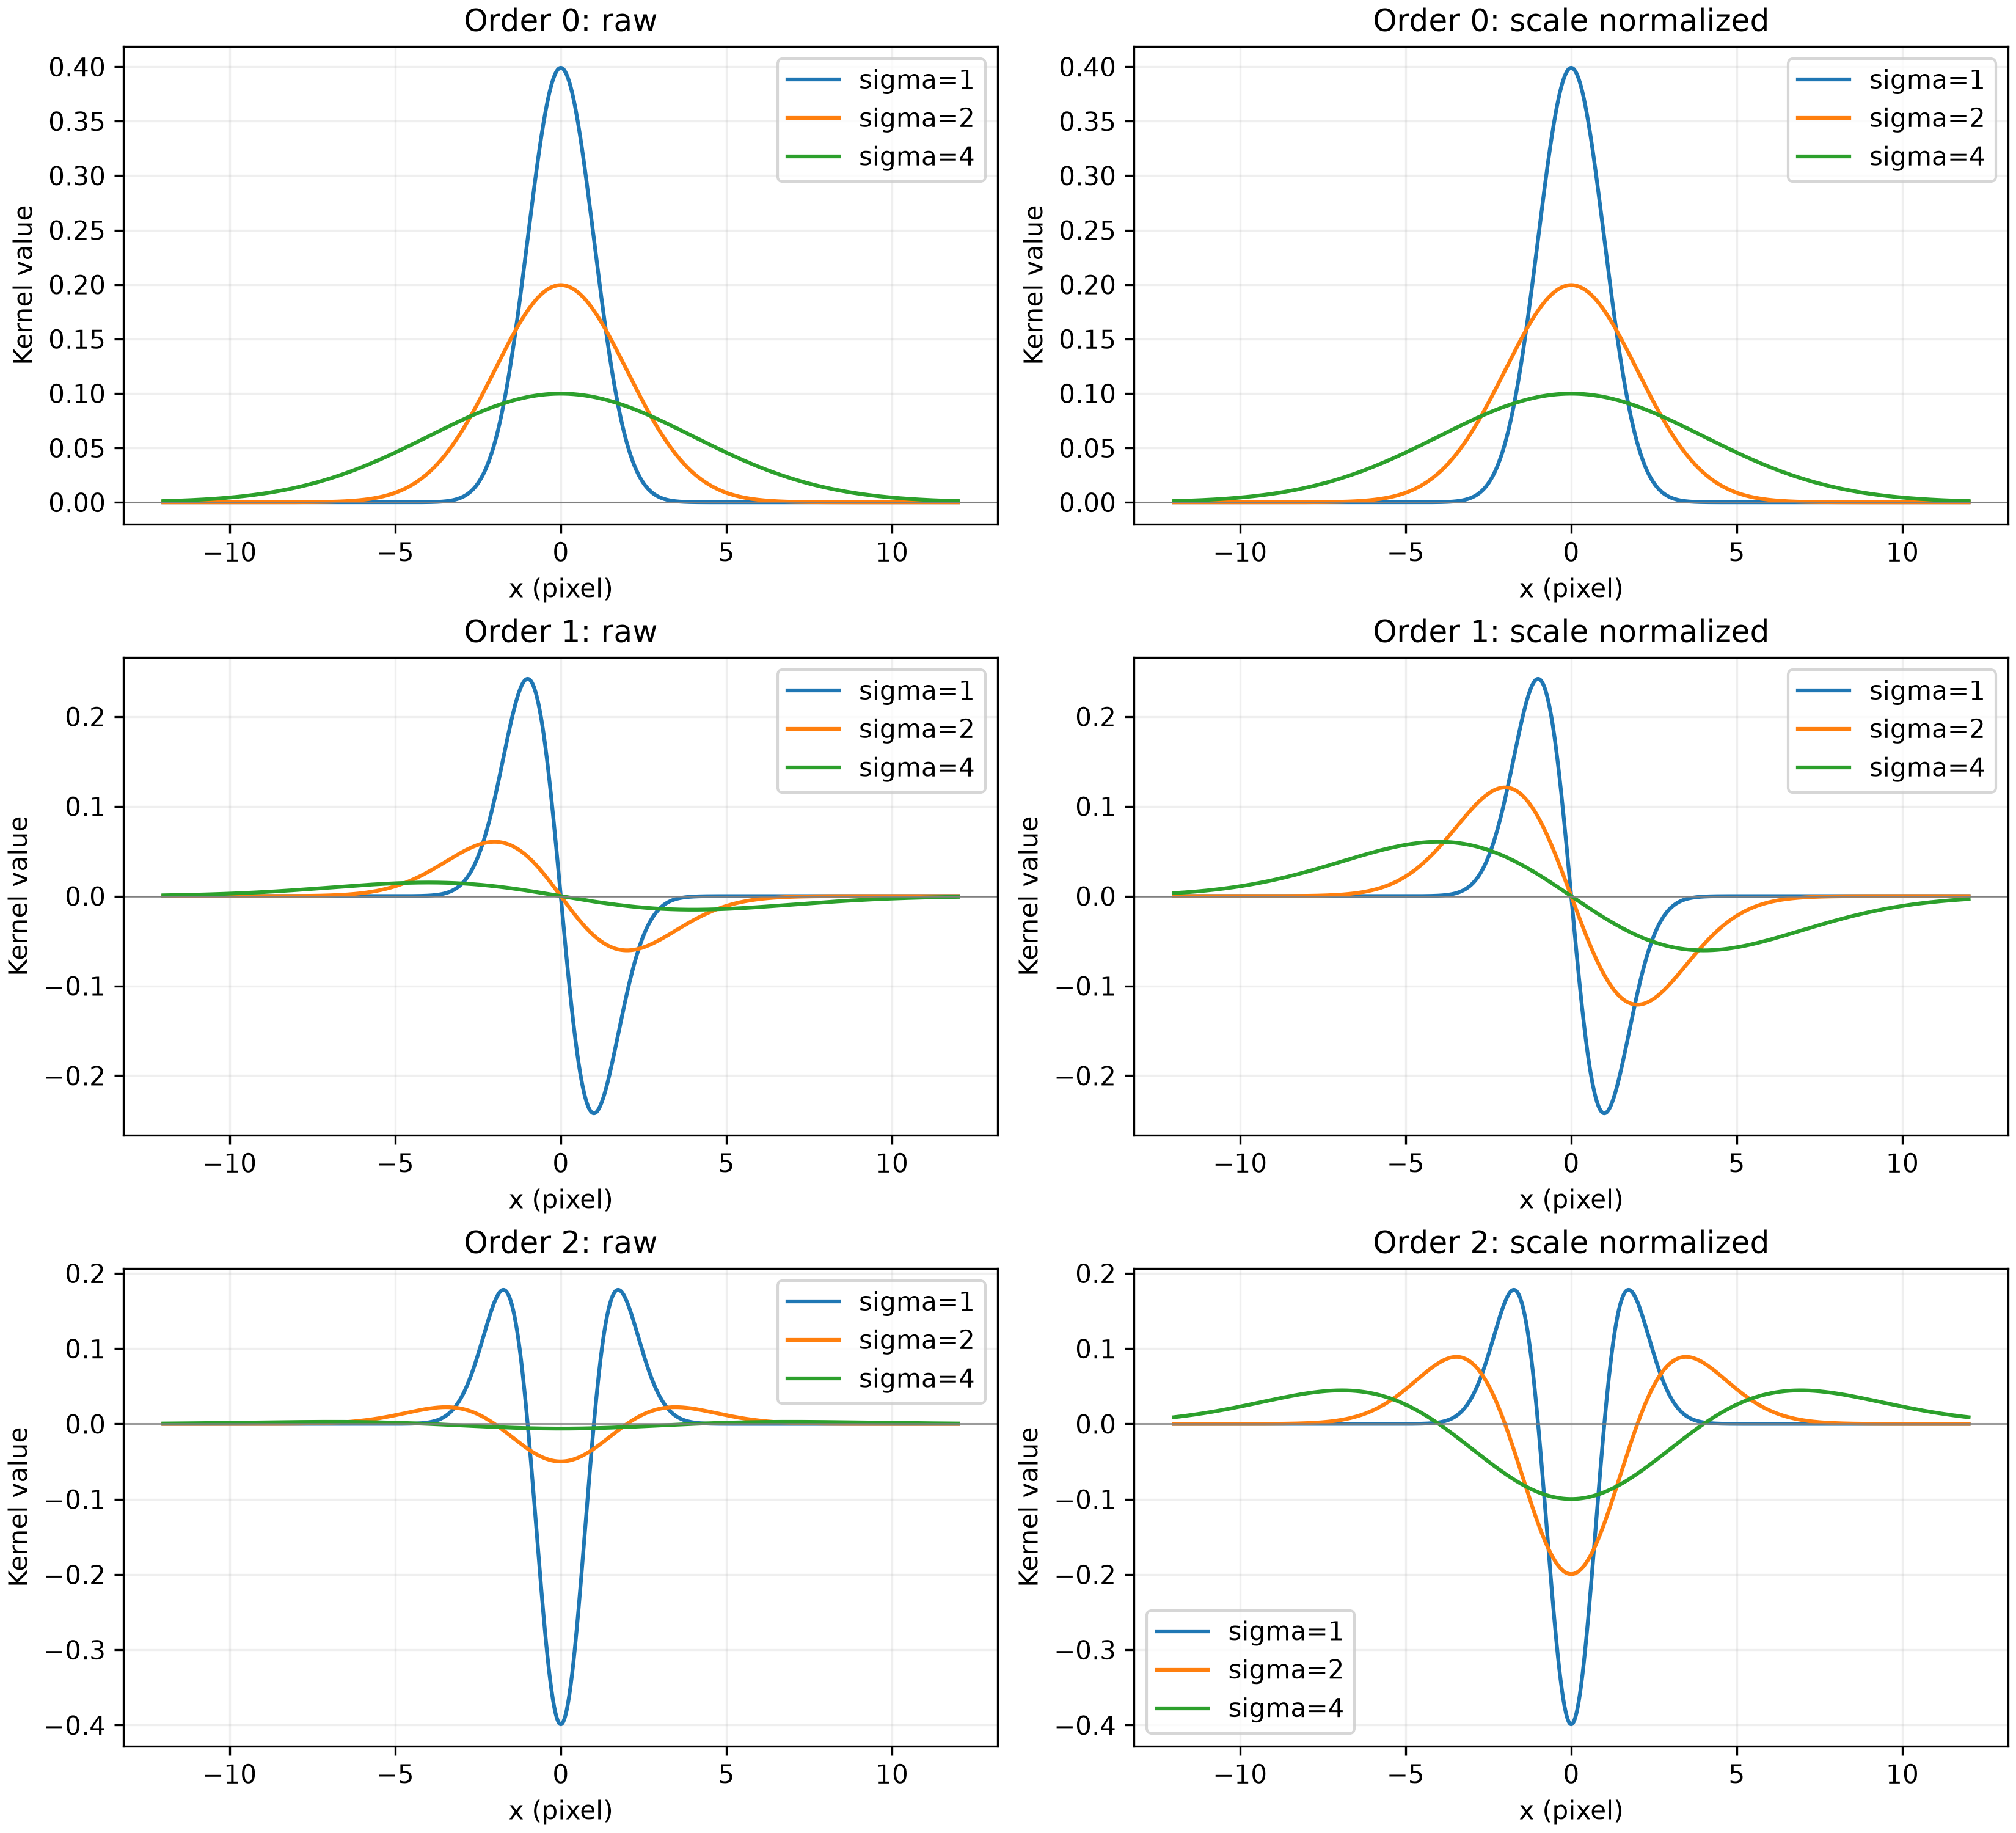
\includegraphics[width=0.90\textwidth]{figures/theory_gaussian_derivatives.png}
\caption{Minh họa giải tích Gaussian và đạo hàm bậc 1, 2 tại ba tỷ lệ. Cột trái là kernel thô, cột phải nhân $\sigma^n$ theo bậc đạo hàm. Đây là đồ thị tính từ công thức, không phải đầu ra thực nghiệm của Fiji.}
\label{fig:analytic_kernels}
\end{figure*}

\subsection{Scale-space: biểu diễn ảnh theo tỷ lệ}
Scale-space là họ ảnh $\{L(\cdot,\cdot;\sigma)\}_{\sigma>0}$, không chỉ là một ảnh đã làm mịn. Ở tỷ lệ nhỏ, các chi tiết mảnh có thể tạo đáp ứng nổi bật; ở tỷ lệ lớn, các nhóm chi tiết có thể được quan sát như một cấu trúc lớn hơn. Cùng một cảnh có thể cần nhiều tỷ lệ vì biên lớn, mạch nhỏ và cụm tế bào không có cùng kích thước \cite{witkin1983scale,lindeberg1994scale}.

\subsubsection{Tính bán nhóm}
Gaussian thỏa mãn
\begin{equation}
G_{\sigma_1}*G_{\sigma_2}
=G_{\sqrt{\sigma_1^2+\sigma_2^2}}.
\end{equation}
Do đó, nếu đã có ảnh tại $\sigma_1$ và muốn tới $\sigma_2>\sigma_1$, mức làm mịn bổ sung trong mô hình liên tục là $\sqrt{\sigma_2^2-\sigma_1^2}$. Hai lần làm mịn với $\sigma=2$ cho tỷ lệ tổng $\sqrt8$, không phải $\sigma=4$. Quan hệ này giải thích vì sao phải quản lý phương sai khi xây dựng nhiều mức tỷ lệ.

\subsubsection{Liên hệ với phương trình truyền nhiệt}
Đặt $t=\sigma^2$. Họ ảnh Gaussian giải phương trình
\begin{equation}
\frac{\partial L}{\partial t}=\frac12\nabla^2L,\qquad L(x,y;0)=I(x,y).
\end{equation}
Mô hình này làm giảm độ tương phản của các cấu trúc nhỏ dần theo $t$. Tính không tăng cường cực trị cục bộ là một cơ sở quan trọng của scale-space Gaussian; không nên suy diễn rằng mọi cấu trúc phát hiện trong ảnh 2D luôn giữ nguyên số lượng hay vị trí qua các tỷ lệ.

\subsubsection{Chọn lưới tỷ lệ}
Repo dùng $\Sigma=\{1,2,4,8\}$ cho đối chiếu cơ bản và lưới dày hơn $\{1,1.4,2,2.8,4,5.7,8\}$ cho Blobs. Lưới hình học cho khoảng cách tương đối gần nhau giữa các kích thước. Lưới thưa giảm thời gian, nhưng có thể bỏ lỡ cực trị theo tỷ lệ nằm giữa hai mức. Lưới dày tăng khả năng định vị kích thước, đồng thời tăng chi phí và số ứng viên cần khử trùng.

\subsection{Đạo hàm Gaussian bậc nhất}
Tính tuyến tính cho phép chuyển đạo hàm sang kernel:
\begin{equation}
L_x=I*\partial_xG_\sigma,\qquad L_y=I*\partial_yG_\sigma.
\end{equation}
Các kernel một chiều tương ứng là
\begin{align}
g'_\sigma(x)&=-\frac{x}{\sigma^2}g_\sigma(x),\\
G_{\sigma,x}(x,y)&=g'_\sigma(x)g_\sigma(y),\\
G_{\sigma,y}(x,y)&=g_\sigma(x)g'_\sigma(y).
\end{align}
Kernel bậc nhất là hàm lẻ, có tổng liên tục bằng 0. Vì vậy ảnh hằng phải cho đạo hàm gần 0; sai khác có hệ thống trên ảnh hằng là một dấu hiệu lỗi chuẩn hóa, đệm biên hoặc cài đặt.

$L_x$ đo biến thiên theo phương ngang nên thường nổi bật tại biên đứng; $L_y$ đo biến thiên theo phương dọc nên thường nổi bật tại biên ngang. Dấu đáp ứng cho biết hướng tăng hoặc giảm cường độ theo trục đã quy ước. Bản đồ có dấu cần được lưu dưới dạng số thực, thay vì chuyển về ảnh 8-bit trước khi đối chiếu.

\subsubsection{Ví dụ biên bước}
Xét biên đứng lý tưởng $I(x)=A\,H(x)$, trong đó $H$ là hàm bước. Sau làm mịn,
\begin{equation}
L(x;\sigma)=A\Phi(x/\sigma),\quad
L_x(x;\sigma)=\frac{A}{\sqrt{2\pi}\sigma}e^{-x^2/(2\sigma^2)}.
\end{equation}
Đạo hàm đạt cực đại ở vị trí biên $x=0$. Khi tăng $\sigma$, đỉnh đáp ứng thấp hơn và rộng hơn; điều này giải thích vì sao gradient lớn không tự động tạo ra một đường biên mảnh. Bước NMS trong Canny giữ lại cực đại theo phương gradient để cải thiện định vị.

\subsection{Gradient: cường độ và hướng biến thiên}
Vector gradient và độ lớn của nó là
\begin{equation}
\nabla L=\begin{bmatrix}L_x\\L_y\end{bmatrix},\quad
M=\sqrt{L_x^2+L_y^2},\quad
\theta=\operatorname{atan2}(L_y,L_x).
\end{equation}
Gradient chỉ theo phương tăng cường độ nhanh nhất; tiếp tuyến của biên lý tưởng vuông góc với gradient. Hàm atan2 sử dụng dấu của cả hai thành phần nên xác định đúng góc phần tư và xử lý trường hợp $L_x=0$ tốt hơn biểu thức $\arctan(L_y/L_x)$.

Độ lớn gradient là bất biến đối với việc quay hệ trục trong mô hình liên tục. Tuy nhiên, cài đặt trên lưới pixel, phép nội suy và lượng tử hóa hướng có thể tạo sai khác theo góc. Trong vùng đồng nhất, khi $M$ gần 0, hướng gradient trở nên nhạy với nhiễu và không nên được diễn giải như một hướng cấu trúc đáng tin cậy.

\subsection{Đạo hàm bậc hai và Laplacian}
Đạo hàm bậc hai một chiều có dạng
\begin{equation}
g''_\sigma(x)=\left(\frac{x^2}{\sigma^4}-\frac1{\sigma^2}\right)g_\sigma(x).
\end{equation}
Trong ảnh hai chiều,
\begin{align}
L_{xx}&=I*(g''_\sigma(x)g_\sigma(y)),\\
L_{yy}&=I*(g_\sigma(x)g''_\sigma(y)),\\
L_{xy}&=I*(g'_\sigma(x)g'_\sigma(y)).
\end{align}
Các đại lượng này đo sự thay đổi của độ dốc, cung cấp thông tin về độ cong mà đạo hàm bậc nhất chưa mô tả đầy đủ. $L_{xy}$ phản ánh sự tương tác giữa hai phương và cần thiết để phân tích các cấu trúc nghiêng.

Laplacian là tổng hai đạo hàm thuần:
\begin{equation}
\nabla^2L=L_{xx}+L_{yy}.
\end{equation}
Đây là một đại lượng vô hướng, hữu ích cho blob và phân tích điểm đổi dấu. Tuy nhiên, hai ma trận Hessian khác nhau có thể có cùng tổng trị riêng; Laplacian một mình không đủ phân biệt cấu trúc dạng đường, dạng đốm hay điểm yên ngựa.

\subsection{Ma trận Hessian và hình học cục bộ}
Khai triển Taylor của ảnh quanh điểm $\mathbf p$ theo độ lệch $\mathbf h$ cho
\begin{equation}
L(\mathbf p+\mathbf h)\approx
L(\mathbf p)+\nabla L^\top\mathbf h+
\frac12\mathbf h^\top\mathcal H\mathbf h,
\end{equation}
với
\begin{equation}
\mathcal H=
\begin{bmatrix}L_{xx}&L_{xy}\\L_{xy}&L_{yy}\end{bmatrix}.
\end{equation}
Do Hessian đối xứng, hai vector riêng có thể được chọn trực giao và trị riêng là số thực. Theo một vector đơn vị $\mathbf v$, đạo hàm bậc hai có hướng là $\mathbf v^\top\mathcal H\mathbf v$. Hai trị riêng chính là các độ cong cực trị của dạng toàn phương này:
\begin{equation}
\lambda_\pm=\frac{L_{xx}+L_{yy}}2
\pm\sqrt{\left(\frac{L_{xx}-L_{yy}}2\right)^2+L_{xy}^2}.
\end{equation}

\subsubsection{Ý nghĩa dấu và độ lớn}
Tại một cực đại sáng cục bộ, cả hai độ cong thường âm; tại cực tiểu tối, chúng thường dương. Với ridge sáng, độ cong ngang thân âm mạnh và độ cong dọc thân nhỏ; với rãnh tối, dấu độ cong ngang thân đảo lại. Trường hợp hai trị riêng trái dấu tương ứng hình học yên ngựa. Các mô tả này áp dụng cho đáp ứng cục bộ ở tỷ lệ đang khảo sát, không phải một bộ phân loại hoàn chỉnh chỉ dựa vào dấu.

Thứ tự trị riêng cần được ghi rõ: FeatureJ ở cấu hình đối chiếu dùng thứ tự đại số $\lambda_+\geq\lambda_-$; Frangi thường sắp theo $|\lambda_1|\leq|\lambda_2|$. Sắp xếp theo trị tuyệt đối không có nghĩa thay trị riêng bằng trị tuyệt đối: dấu vẫn phải được giữ để chọn ridge sáng hay tối.

\subsubsection{Ví dụ kiểm tra bằng ảnh đa thức}
Với $I(x,y)=ax^2+2bxy+cy^2+dx+ey+f$, ta có
\begin{equation}
\nabla I=\begin{bmatrix}2ax+2by+d\\2bx+2cy+e\end{bmatrix},
\quad
\mathcal H_I=\begin{bmatrix}2a&2b\\2b&2c\end{bmatrix}.
\end{equation}
Trong miền liên tục không biên, làm mịn thêm hằng số $\sigma^2(a+c)$ vào ảnh nhưng không đổi Hessian. Vì vậy ảnh đa thức là một ví dụ hữu ích để kiểm tra dấu, thứ tự trục và đáp ứng bậc hai. Trên ảnh hữu hạn, cần loại vùng chịu ảnh hưởng của đệm biên.

\subsection{Chuẩn hóa đạo hàm theo tỷ lệ}
Để so sánh đáp ứng giữa các tỷ lệ, đạo hàm tổng bậc $n$ được chuẩn hóa bởi
\begin{equation}
L_{x^my^k,\gamma}=\sigma^{(m+k)\gamma}L_{x^my^k},\quad n=m+k.
\end{equation}
Với $\gamma=1$, đạo hàm bậc nhất nhân $\sigma$ và đạo hàm bậc hai nhân $\sigma^2$ \cite{lindeberg1998feature}. Ví dụ biên bước cho $\sigma L_x(0;\sigma)=A/\sqrt{2\pi}$: biên độ chuẩn hóa tại đỉnh không còn giảm chỉ vì tăng $\sigma$.

Chuẩn hóa giúp so sánh cấu trúc ở nhiều kích thước, nhưng không đảm bảo mọi ảnh và mọi dạng đối tượng đều có cùng độ nhạy. Cần phân biệt hai loại phép đo: đối chiếu toán tử thô với FeatureJ phải dùng cùng cờ chuẩn hóa; phát hiện đa tỷ lệ có thể chủ động dùng đáp ứng chuẩn hóa. Chuẩn hóa hai lần sẽ tạo hệ số sai lệch phụ thuộc $\sigma$.

\subsection{Structure Tensor: tổng hợp định hướng trong lân cận}
Hessian dùng đạo hàm bậc hai tại một tỷ lệ. Structure Tensor tổng hợp tích các đạo hàm bậc nhất trong một vùng:
\begin{equation}
\mathcal S_{\sigma_d,\sigma_i}
=G_{\sigma_i}*
\begin{bmatrix}
L_x^2&L_xL_y\\L_xL_y&L_y^2
\end{bmatrix}_{\sigma_d}.
\end{equation}
$\sigma_d$ điều khiển tỷ lệ tính gradient, còn $\sigma_i$ điều khiển vùng tích phân hướng. Tăng $\sigma_i$ làm hướng ổn định hơn trong vùng nhiễu, nhưng cũng có thể gộp nhiều cấu trúc có hướng khác nhau.

Với mọi $\mathbf v$, $\mathbf v^\top\mathcal S\mathbf v$ là trung bình có trọng số của $(\mathbf v^\top\nabla L)^2$, nên $\mathcal S$ bán xác định dương. Hai trị riêng $\mu_1\geq\mu_2\geq0$ được diễn giải như sau: cả hai nhỏ biểu thị vùng gần đồng nhất; $\mu_1$ lớn và $\mu_2$ nhỏ biểu thị một hướng biến thiên ưu thế; cả hai lớn thường xuất hiện ở góc hoặc vùng kết cấu nhiều hướng.

\begin{equation}
C=\frac{\mu_1-\mu_2}{\mu_1+\mu_2+\epsilon}
\end{equation}
là một độ đo coherence thường dùng. $C$ cao chỉ hữu ích khi năng lượng gradient đủ lớn; vùng rất tối hoặc đồng nhất có thể tạo tỷ số thiếu ổn định nếu bỏ $\epsilon$. Vector riêng ứng với $\mu_1$ gần hướng pháp tuyến của cấu trúc dạng đường, còn hướng tiếp tuyến tương ứng phương còn lại. Vì tensor dùng tích gradient, đảo tương phản không làm đổi nó như đối với dấu Hessian.

\subsection{Từ đặc trưng vi phân đến ba bài toán phát hiện}
\subsubsection{Biên: gradient, NMS và hysteresis}
Canny bắt đầu bằng đạo hàm của ảnh làm mịn, tính $M,\theta$, rồi thực hiện NMS và phân ngưỡng kép \cite{canny1986computational}. NMS giữ các điểm có $M$ cực đại cục bộ theo pháp tuyến biên. Hysteresis giữ điểm mạnh $M\geq T_h$ và điểm yếu $T_l\leq M<T_h$ nếu có đường liên thông tới điểm mạnh. Ngưỡng quá thấp giữ nhiều kết cấu nền; ngưỡng quá cao bỏ sót biên có tương phản yếu.

Gradient mạnh phản ánh thay đổi cường độ, còn nhãn đường biên của con người thường gắn với đối tượng. Vì thế biên do bóng, nhiễu kết cấu hoặc vân nền có thể bị thuật toán giữ lại nhưng không được người gán nhãn xem là đường bao cần thiết. Đây là một nguyên nhân khiến đối chiếu số học tốt chưa kéo theo F1 phát hiện cao.

\subsubsection{Ridge: phân tích độ cong ngang và dọc}
Một mô hình ridge sáng thẳng là $I(x,y)=A\exp[-x^2/(2s^2)]$, không đổi theo $y$. Gần tâm ridge, $L_{xx}$ âm và $L_{yy}$ gần 0; độ cong lớn nằm theo phương ngang thân. Với ridge tối trên nền sáng, dấu đảo lại. Mạch máu trong ảnh DRIVE được xem là cấu trúc tối, nên lựa chọn cực tính phải phù hợp.

Frangi dùng tỷ số $R_B=|\lambda_1|/(|\lambda_2|+\epsilon)$ và độ mạnh $S=\sqrt{\lambda_1^2+\lambda_2^2}$ sau chuẩn hóa tỷ lệ \cite{frangi1998multiscale}. $R_B$ nhỏ gợi ý cấu trúc dài; thừa số theo $S$ giảm đáp ứng ở nền ít cấu trúc. Lấy cực đại theo $\sigma$ giúp tổng hợp các mạch khác độ rộng, song còn cần ngưỡng, mặt nạ FOV và cách đánh giá vùng phân đoạn.

\subsubsection{Blob: cực trị đồng thời theo vị trí và tỷ lệ}
Đáp ứng $R(x,y,\sigma)=\sigma^2|\nabla^2L|$ được tìm cực đại theo cả không gian và tỷ lệ. Dấu của Laplacian trước phép lấy trị tuyệt đối giúp chọn blob sáng hoặc tối. Nếu chỉ tìm cực đại 2D độc lập ở từng mức, cùng một đối tượng có thể được đếm nhiều lần.

Với blob Gaussian lý tưởng $I=A\exp[-(x^2+y^2)/(2s^2)]$, tại tâm ta có
\begin{equation}
\sigma^2|\nabla^2L(0,0;\sigma)|
=\frac{2As^2\sigma^2}{(s^2+\sigma^2)^2}.
\end{equation}
Biểu thức đạt cực đại tại $\sigma=s$, cho một ví dụ giải tích về lựa chọn tỷ lệ đặc trưng. Quy ước $R\approx\sqrt2\sigma$ thường dùng để vẽ vòng tròn biểu diễn blob trong 2D; đây là ánh xạ kích thước theo mô hình, không phải đẳng thức bán kính thật cho mọi dạng tế bào.


\begin{figure}[htbp]
\centering
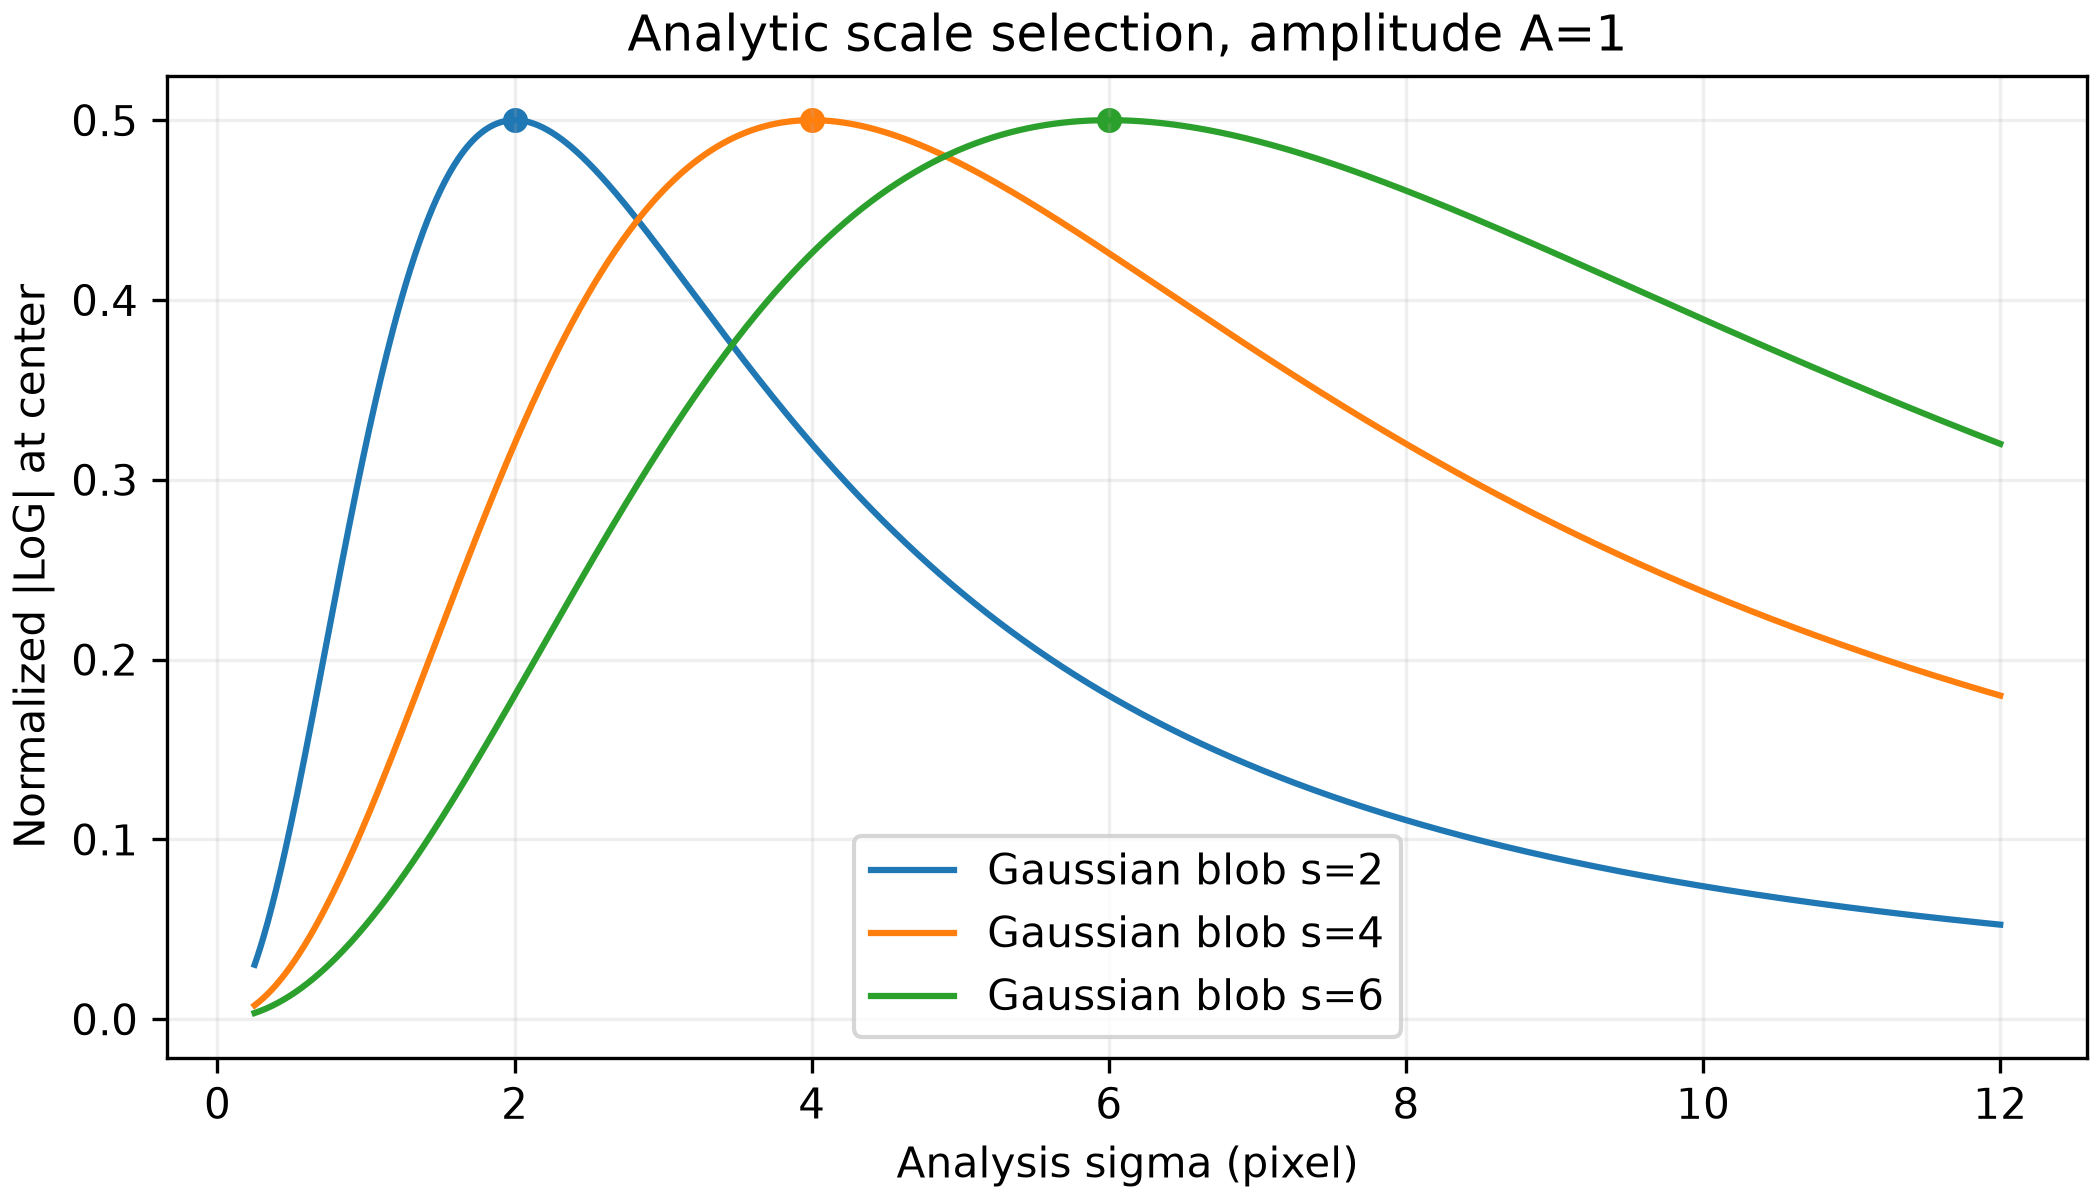
\includegraphics[width=\columnwidth]{figures/theory_blob_scale_selection.png}
\caption{Chọn tỷ lệ trên mô hình blob Gaussian biên độ 1: đáp ứng LoG chuẩn hóa tại tâm đạt cực đại khi $\sigma=s$. Đồ thị là ví dụ giải tích để giải thích nguyên lý chọn kích thước.}
\label{fig:analytic_blob_scale}
\end{figure}

\subsection{Tổng hợp ý nghĩa các bản đồ}
\begin{table*}[t]
\centering
\caption{Vai trò của các đại lượng vi phân và điểm cần lưu ý khi diễn giải}
\begin{tabularx}{\textwidth}{lXX}
\toprule
Đại lượng & Thông tin chính & Giới hạn khi sử dụng\\
\midrule
$L$ & Cường độ ở tỷ lệ $\sigma$ & Làm mịn mạnh có thể mất chi tiết nhỏ\\
$L_x,L_y$ & Biến thiên có hướng và có dấu & Phụ thuộc trục và quy ước tích chập\\
$\|\nabla L\|$ & Mức biến thiên tổng hợp & Biên mạnh có thể là kết cấu nền\\
$L_{xx},L_{yy},L_{xy}$ & Độ cong cục bộ & Nhạy với rời rạc hóa và nhiễu\\
$\mathcal H,\lambda_1,\lambda_2$ & Hình học ridge/blob, hướng độ cong & Phải thống nhất thứ tự và cực tính\\
$\sigma^2\nabla^2L$ & Đáp ứng blob chuẩn hóa & Cần cực trị theo tỷ lệ và khử trùng\\
$\mathcal S,\mu_1,\mu_2$ & Năng lượng, hướng biến thiên trong vùng & Coherence cao cần đi kèm năng lượng đủ lớn\\
\bottomrule
\end{tabularx}
\end{table*}
Các bản đồ trên tạo một chuỗi phân tích: Gaussian xác định tỷ lệ quan sát; đạo hàm đo biến thiên; gradient, Hessian và tensor cô đọng thông tin; bộ dò cùng bước hậu xử lý chuyển thông tin liên tục thành biên, vùng mạch hoặc danh sách blob.
